\usetikzlibrary{arrows}


\section{Общее определение вероятностного пространства.}

\subsection{Теория меры в слабой форме.}
\textbf{Attention!!!} Вплодь до определения случайной величины в общем случае конспект будет содержать исключительно
сухие формулировки, факты и утверждения без доказательств, и моих комментариев. Это связано с тем, что практически всё что есть
в этой части курса мной подробно разобрано и расписано в \href{https://raw.githubusercontent.com/johanDDC/My_TeXs/5981fbe92fbd8dfae37ea2c29fbf204a942d0d09/pdf/Lebeg/Lebeg.pdf}{моём конспекте по теории меры Лебега}.
Там представлено действительно много примеров на эти темы, в частности там можно попытаться дейтсвительно вникнуть в то,
что такое Борелевская алгебра. Конспект пока не закончен и на половину, но сейчас там уже есть всё, что нам
преподносилось в этой части курса.

Пусть множество $X$ не пусто.
\begin{definition}
    \it{Алгеброй подмножеств множества $X$} (алгеброй) называется набор $\mathcal{A} \subset 2^X$, если выполнены следующие свойства:
    \begin{enumerate}
        \item $X, \nothing \in \mathcal{A}$.
        \item $A, B \in \mathcal{A} \implies A \setminus B, A \cap B, A \cup B \in \mathcal{A}$.
    \end{enumerate}
\end{definition}
\begin{definition}
    \it{$\sigma$-алгеброй} называется набор $\mathcal{A} \subset 2^X$, если выполнены следующие свойства:
    \begin{enumerate}
        \item $\mathcal{A}$ является алгеброй.
        \item Если множества $A_1, A_2, \ldots \in \mathcal{A}$, то их счётные объединение и пересечение также
        там лежат: $\bigcap_{j = 0}^{\infty} A_j \in \mathcal{A}, \bigcup_{j = 0}^{\infty} A_j \in \mathcal{A}$
    \end{enumerate}
\end{definition}
Пусть $S$ --- какой-то набор подмножеств множества $X$.
\begin{definition}
    $\sigma(S)$ называется $\sigma$-алгеброй, \it{порождённой} $S$. $\sigma(S)$ есть пересечение всех
    $\sigma$-алгебр, содержащих $S$.
\end{definition}
Пусть $\mathcal{A}$ --- алгебра множеств.
\begin{definition}
    Функция $P \colon \mathcal{A} \to [0, 1]$ называется \it{аддитивной}, если для произвольных $A, B \in \mathcal{A},
    A \cap B = \nothing$ выполнено
    \[
        P(A \cup B) = P(A) + P(B)
    \]
    Функция $P \colon \mathcal{A} \to [0, 1]$ называется \it{счётно-аддитивной}, если для произвольного, не более чем
    счётного набора $A_n \in \mathcal{A}$, такого что $\bigcup_{n = 1}^{\infty} A_n \in  \mathcal{A}$ выполнено
    \[
        P \left( \bigcup_{n = 1}^{\infty} A_n \right) = \sum\limits_{n=1}^{\infty} P(A_n)
    \]
\end{definition}
Пусть теперь $\mathcal{A}$ --- $\sigma$-алгебра.
\begin{definition}
    Счётно-аддитивная функция $P \colon \mathcal{A} \to [0, 1]$ называется \it{вероятностной мерой} на $\mathcal{A}$,
    если $P(\Omega) = 1$.
\end{definition}
\begin{definition}
    Тройка $\left( \Omega, \mathcal{A}, P \right)$ называется \it{вероятностным пространством}.
\end{definition}
\begin{proposal}
    Пусть $P \colon \mathcal{A} \to [0, 1]$ --- аддитивная функция на алгебре $\mathcal{A}$. Функция $P$ счётно-аддитивна
    на $\mathcal{A}$ тогда и только тогда, когда для всякого набора $A_n \in \mathcal{A}$, такого, что каждое следующее
    множество вложено в предыдущее ($A_{n + 1} \subset A_n$), и $\bigcup_{n=1}^{\infty} A_n = \nothing$ выполнено
    $\lim P(A_n) = 0$.
\end{proposal}
\begin{theorem}
    Пусть $\mathcal{A}$ --- некоторая алгебра подмножеств пространства $\Omega$, и пусть $P_0 \colon \mathcal{A} \to
    [0, 1]$ --- счётно-аддитивная функция множества на алгебре $\mathcal{A}$. Тогда существует единственная вероятностная мера
    $P \colon \sigma(\mathcal{A}) \to [0, 1]$, такая что $P\Big|_{\mathcal{A}} = P_0$.
\end{theorem}

\subsection{Случайная величина в общем случае.}
Пусть у нас есть вероятностное пространство: $(\Omega, \mathcal{A}, P)$. Заметим такую вещь, как только множество
$\Omega$ стало произвольным, мы начали испытывать некие проблемы с определением события. Если в конечном и счётном
случаях мы называли событиями вообще всякое подмножество в $\Omega$, то теперь так не получится, в частности потому что
если $A, B$ --- события, то нам бы хотелось, чтобы событиями являлись так же $A \cap B, A \cup B, A \setminus B$, а это
не всегда возможно, когда мы говорим о континуальных множествах. Чтобы такие ограничения обойти мы придумали какую-то науку
и создали \it{алгебры}. С алгебрами жить становится веселее, т.к. для множеств из алгебры все наши желания исполняются.
\it{$\sigma$-алгебры} вообще являются пределом мечтаний, и элементы $\sigma$-алгебр мы уже можем воспринимать как полноценные
события. Действительно, что бы мы с ними не делали, мы снова получим элемент из $\sigma$-алгебры, т.е. снова получим событие.

Теперь нам нужно ввести понятние случайной величины. В конечном и счётном случае случайные величины у нас отображали
всевозможные события в числа. Сейчас идея будет примерно та же самая, с поправкой на новое определение события.
\begin{definition}
    Произвольная функция $X \colon \Omega \to \RR$ называется \it{случайной величиной}, тогда и только тогда, когда
    для всякого $t \in \RR$ выполняется
    \[
        \{w \in \Omega \colon X(w) \leq t\} \in \mathcal{A}
    \]
    Т.е. $X$ --- случайная величина, тогда и только тогда, когда множество $\{w \colon X(w) \leq t\}$ является событием $\forall ~ t$.
\end{definition}
\begin{comment}
    Заметим следующее:
    \[
        \{w \in \Omega \colon X(w) \leq t\} = \{w \in \Omega \colon X(w) \in (-\infty; t]\}
    \]
    Т.е. то множество, которое мы хотим считать событием при любом $t$ состоит из исходов, которые под действием случайной
    величины $X$ попадают в множество $(-\infty; t]$. Т.е. это множество по определению является полным прообразом множества
    $\{X(w) \colon X(w) \in (-\infty; t]\} = X((-\infty; t])$, и мы соответственно его будет обозначать как $X^{-1}((-\infty; t])$.
\end{comment}
Теперь постараемся расширить наше определение. Перепишем его в следующем виде: $X$ --- случайная величина $\iff
\{w \colon X(w) \in B\}$. По определению мы умеем найти вероятность такого события когда $B = (-\infty, t] ~ \forall ~ t$.
Но мы хотим как-то расширить класс $B$ чтобы считать вероятности более сложных событий.

Пусть $X$ --- случайная величина.
\label{random_val_for_Borelian}
\begin{proposal}
    Тогда для всякого $B \in \mathcal{B}(\RR)$ множество
    $\{w \colon X(w) \in B\} = X^{-1}(B) \in \mathcal{A}$.
\end{proposal}
\begin{proof}
    Свойства полного прообраза:
    \begin{itemize}
        \item $X^{-1}\left( \bigcap_{k=1}^{\infty} A_n \right) = \bigcap_{k=1}^{\infty} X^{-1}(A_n)$.
        \item $X^{-1}\left( \bigcup_{k=1}^{\infty} A_n \right) = \bigcup_{k=1}^{\infty} X^{-1}(A_n)$.
        \item $X^{-1} (\Omega \setminus B) = \RR \setminus X^{-1} (B)$.
    \end{itemize}
    Рассмотрим систему множеств $C = \{B \subset \RR \colon X^{-1}(B) \in \mathcal{A}\}$. $\mathcal{C}$ состоит из таких
    множеств, прообразы которых лежат в $\sigma$-алгебре $A$. Проверим, что $\mathcal{C}$ является $\sigma$-алгеброй, и
    содержит все лучи вида $(-\infty, t]$. После того как мы это проверим, то т.к.
    $\mathcal{B}(\RR) = \sigma((-\infty, t])$ (доказывалось в пункте 2.3 \href{https://raw.githubusercontent.com/johanDDC/My_TeXs/5981fbe92fbd8dfae37ea2c29fbf204a942d0d09/pdf/Lebeg/Lebeg.pdf}{конспекта по мере Лебега}),
    мы получим включение $\mathcal{B}(\RR) \subset \mathcal{C}$, т.е. мы будем знать,
    что прообраз любого Борелевского множества (по определению $\mathcal{C}$) лежит в $\mathcal{A}$, а это именно то,
    что мы хотим доказать.\\
    Прежде всего покажем, что $\mathcal{C}$ --- $\sigma$-алгебра:
    \begin{align*}
        &X^{-1}(\nothing) = \nothing \in \mathcal{A} \implies \nothing \in \mathcal{C}, ~~~
        X^{-1}(\RR) = \Omega \in \mathcal{A} \implies \Omega \in \mathcal{C}\\
        &B \in \mathcal{C} \iff X^{-1}(B) \in \mathcal{A} \implies \Omega \setminus X^{-1}(B) \in \mathcal{A}
        \iff X^{-1}(\RR \setminus B) \in \mathcal{A} \iff \RR \setminus B \in \mathcal{C}\\
        &B_n \in \mathcal{C} \iff X^{-1}(B_n) \in \mathcal{A} \implies \bigcap_{k=1}^{\infty} X^{-1}(B_n),
        \bigcup_{k=1}^{\infty} X^{-1}(B_n) \in \mathcal{A} \iff X^{-1}\left( \bigcap_{k=1}^{\infty} B_n \right),
        X^{-1}\left( \bigcup_{k=1}^{\infty} B_n \right) \in \mathcal{A} \iff\\
        &\iff \bigcap_{k=1}^{\infty} B_n, \bigcup_{k=1}^{\infty} B_n \in \mathcal{C}
    \end{align*}
    Таким образом $\mathcal{C}$ --- $\sigma$-алгебра. Кроме того из условия следует, что $\mathcal{C}$ содержит прообразы
    лучей, т.к. $X$ --- случайная величина по условию. Таким образом имеем $\mathcal{B}(\RR) \subset \mathcal{C}$.
\end{proof}
\begin{designation}
    Введём обозначение, аналогичное обозначению, которое мы вводили для дискретного случая. Если $X$ --- случайная
    величина, то
    \[
        \{X \leq t\} \iff \{w \in \Omega \colon X(w) \leq t\} = X^{-1}((-\infty, t])
    \]
\end{designation}

Пусть теперь $X, Y$ --- случайные величины, $a, b \in \RR$.

\begin{proposal}
    Выражения $aX + bY, X \cdot Y$ являются случайными величинами.
\end{proposal}
\begin{proof}
    Если $X = const$, то $X$, очевидно, является случайной величиной. Рассмотрим выражение $aX$:
    \[
        \{aX \leq t\} =
        \begin{cases}
            \left\{ X \leq \frac{t}{a} \right\} \in \mathcal{A} & a > 0\\
            \left\{ X \geq -\frac{t}{a} \right\} \in \mathcal{A} & a < 0\\
        \end{cases}
    \]
    Таким образом выражение $aX$ является случайной величиной. Рассмотрим теперь выражение $X + Y$. Покажем, что
    $X + Y > t$ является событием:
    \[
        \{X + Y > t\} = \{X > t - Y\} = \bigcup_{r_n \in \QQ} \left( \{X > r_n\} \cap \{r_n > t - Y\} \right)
    \]
    Т.к. $\{X > r_n\}$ --- дополнение к $\{X \leq r_n\} \in \mathcal{A}$, то $\{X > r_n\} \in \mathcal{A}$.\\
    Т.к. $\{r_n > t - Y\}$ --- дополнение к $\{-Y < r_n - t\} \in \mathcal{A}$, то $\{r_n > t - Y\} \in \mathcal{A}$.\\
    Из этих двух условий следует, что $\{X + Y > t\} \in \mathcal{A} \implies \{X + Y \leq t\} \in \mathcal{A}$
    (как дополнение) $\implies X + Y$ --- случайная величина.\\
    Кроме того понятно, что $X^2$ --- также является случайной величиной, т.к. $\{X^2 \leq t\} =
    X^{-1}([-\sqrt{t}, \sqrt{t}])$, где $[-\sqrt{t}, \sqrt{t}]$ --- Борелевское множество.\\
    Из предыдущих двух утверждений следует, что $X \cdot Y = \frac{(X + Y)^2 - X^2 - Y^2}{2}$ является случайной величиной.
\end{proof}
\begin{proposal}
    Пусть $X_n$ --- случайные величины, и $\forall ~ w \implies \lim X_n(w) = X(w)$. Тогда $X$ --- случайная величина.
    Т.е. поточечный предел случайных величин является случайной величиной.
\end{proposal}
\begin{proof}
    Необходимо показать, что $\forall ~ t \implies \lim X_n(w) \leq t$. Покажем, что $\lim X_n(w) \leq t
    \iff \forall ~ k \in \NN ~ \exists ~ N \in \NN \colon \forall ~ n > N \implies X_n(w) \leq t + \frac{1}{k}$.\\
    $\Rightarrow \colon$ Практически очевидно. Для каждой $\frac{1}{k}$ начиная с некоторого момента $X_n$ попадают
    в окрестность предела. Значит, они отличаются от предела менее чем на $\frac{1}{k} \implies \lim X_n(w) \leq t + \frac{1}{k}$.\\
    $\Leftarrow \colon$ Совсем очевидно. Если с некоторого номера $X_n(w) \leq t + \frac{1}{k}$, то переходим к пределу:
    $\lim X_n(w) \leq t + \frac{1}{k}$ --- верно для любого $k \implies \lim X_n(w) \leq t$.\\
    Перепишем теперь на языке теоретико-множественных операций:
    \[
        \xymatrix{
        {\lim X_n(w) \leq t}\ar@{<=>}[r]\ar@{<->}[d] & {\forall ~ k ~ \exists ~ N \colon \forall ~ n > N \implies X_n(w) \leq t + \frac{1}{k}}\ar@{<->}[d]\\
        {\{w \colon X(w) \leq t\}} \ar@{=}[r]& {\bigcup\limits_{k=1}^{\infty}\bigcap\limits_{N=1}^{\infty}\bigcup\limits_{n=N}^{\infty}
        \left\{w \colon X_n(w) \leq t + \frac{1}{k}\right\}}
        }
    \]
    Остаётся заметить, что правые множества лежат в $\mathcal{A}$.
\end{proof}
\begin{comment}
    Объясняю переход от выражения в кванторах к теоретико-множественной записи: рассмотрим ту же запись, и покажем для парочки
    кванторов. Итак, работаем с записью $\forall ~ k ~ \exists ~ N \colon \forall ~ n > N \implies X_n(w) \leq t + \frac{1}{k}$.
    Логично, что чтобы учесть квантор $\forall ~ k \in \NN$, нужно объединить все множества для всевозможных $k$:
    $\bigcup\limits_{k=1}^{\infty}\left\{w \colon X_n(w) \leq t + \frac{1}{k}\right\}$. Аналогично, чтобы учесть квантор
    существования $\exists ~ N \in \NN$, нужно пересечь все множества для всевозможных $N$:
    $\bigcap\limits_{N=1}^{\infty}\left\{w \colon X_n(w) \leq t + \frac{1}{k}\right\}$. Далее это превращается просто в
    конструктор.
\end{comment}

\subsection{Распределение случайных величин.}
Пусть $X$ --- случайная величина на вероятностном пространстве $(\Omega, \mathcal{A}, P)$.
\begin{definition}
    \it{Распределением} случайной величины $X$ называется вероятностная мера $\mu_X$ на $\mathcal{B}(\RR)$,
    определяемая следующим равенством:
    \[
        \mu_X(B) = P(\{w \colon X(w) \in B\}) = P(X^{-1}(B))
    \]
    По \hyperref[random_val_for_Borelian]{предложению} мы знаем, что $X^{-1}(B)$ (где $B$ ---
    Борелевское множество) лежит в $A$, а значит мы можем брать у него вероятность. Счётная аддитивность $\mu_X$
    следует из счётной аддитивности $P$ и свойств полного прообраза.
\end{definition}
\begin{definition}
    \it{Функцией распределения} случайной величины $X$ называется функция
    \[
        F_X(t) = \mu_X((-\infty, t]) = P(\{X \leq t\})
    \]
\end{definition}
\begin{designation}
    Скобками $\langle a, b \rangle$ будем обозначать любой промежуток от $a$ до $b$, подчёркивая, что
    нам не важно, является ли он отрезком, полуинтервалом или интервалом.
\end{designation}
\begin{proposal}
    Функция распределения $F_X$ удовлетворяет следующим свойствам:
    \begin{enumerate}
        \item $F_X$ не убывает;
        \item $F_X$ непрерывна справа;
        \item $\lim\limits_{t \to -\infty} F_X(t) = 0$ и $\lim\limits_{t \to \infty} F_X(t) = 1$;
    \end{enumerate}
\end{proposal}
\begin{proof}
    1) Пусть $t < s$. Тогда
    \[
        F_X(t) = P((-\infty, t]), ~
        F_X(s) = P((-\infty, s]) = \underbrace{P((-\infty, t])}_{\geq 0}
        + \underbrace{P((t, s])}_{\geq 0} \implies F_X(t) \leq F_X(s)
    \]
    2) Пусть $t_n \geq t$ и $t_n \to t$. Заметим что
    \[
        \bigcap_{k = 1}^{\infty} \{X \leq t + \frac{1}{k}\} = \{X \leq t\}
    \]
    По непрерывности вероятностной меры: $P\left(X \leq t + \frac{1}{k}\right) \to P(X \leq t)$. В частности
    \[
        \forall ~ \epsilon > 0 \exists ~ k \colon P\left(X \leq t + \frac{1}{k}\right) \leq P(X \leq t) + \epsilon
    \]
    И с другой стороны $P\left(X \leq t + \frac{1}{k}\right) \geq P(X \leq t)$. Т.к. $t_n \to t$ и $t_n \geq t$, то
    $\exists ~ n_0 \colon \forall ~ n > n_0 \implies t \leq t_n \leq t + \frac{1}{k}$. В силу монотонности функции распределения:
    $F_X(t) \leq F_X(t_n) \leq F_X\left( t + \frac{1}{k} \right) \leq F_X(t) + \epsilon$. Отсюда по определению предела
    имеем $F_X(t_n) \to F_X(t)$.\\
    3) Доказательство этого пункта аналогично доказательству предыдущего путём устремления $t$ к $-\infty$ или $+\infty$.
\end{proof}
\begin{theorem}
    Пусть дана функция $F \colon \RR \to [0, 1]$ со свойствами 1)-3). Тогда существует вероятностное пространство
    $(\Omega, \mathcal{A}, P)$ и случайная величина $X$ на нём, такая что $F$ является функцией распределения $X$.
    Кроме того распределение случайной величины $\mu_X$ однозначно задаётся функцией распределения $F_X$.
\end{theorem}
\it{Идея доказательства:} Пусть $\mathcal{A}$ --- алгебра всевозможных попарно непересекающихся промежутков
на $\RR$. Нетрудно видеть, что $\sigma(\mathcal{A}) = \mathcal{B}(\RR)$. Пусть $X, Y$ --- две случайные величины,
такие что $F_X = F_Y$. Тогда $\mu_X \Big_{\mathcal{A}} = \mu_Y \Big_{\mathcal{A}}$. И по теореме Лебега $\mu_X = \mu_Y$
на $\sigma(\RR)$.\\
Доказательство первой части чуть менее тривиально: рассмотрим ту же алгебру, и положим
$P(A) = \sum\limits_{j = 1}^{N} F(b_j) - F(a_j), ~ \forall ~ A \in \mathcal{A}$. Заметим, что каждое $A$ выглядит
как $\bigcup_{j = 1}^{N} \langle a_j, b_j \rangle$. Видно, что $P$ --- аддитивна. Если бы мы проверили, что
$P$ так же счётно-аддитивна (что верно), то по теореме Лебега: $\exists! ~ \widetilde{P}$ --- счётно-аддитивная мера
на $\sigma(\mathcal{A}) = \mathcal{B}(\RR)$, такая что $\widetilde{P}\Big_{\mathcal{A}} = P$. И функцией распределения
тождественной случайной величина на $(\RR, \mathcal{B}(\RR), \widetilde{P})$ является $F$.

\subsection{Абсолютно непрерывные и дискретные случайные величины.}
Пусть $(\Omega, \mathcal{A}, P)$ --- вероятностное пространство.
\begin{definition}
    Случайная величина $X$ имеет \it{абсолютно непрерывное распределение}, если существует такая неотрицательная
    и интегрируемая функция $\rho_X$, что
    \[
        F_X(t) = \int\limits_{-\infty}^{t} \rho_X(x) dx
    \]
    При это функция $\rho_X$ называется \it{плотностью} случайной величины $X$.
\end{definition}
Понятно, что
\[
    P(a < X \leq b) = \mu_X((a, b]) = F_X(b) - F_X(a) = \int\limits_{a}^{b} \rho_X(x) dx
\]
Кроме того
\[
    P(X = a) = \lim\limits_{n \to \infty}\left( F_X(a) - F\left( a + \frac{1}{n} \right) \right) = 0
\]
Свойства плотности:
\begin{itemize}
    \item $\rho_X$ неотрицательна;
    \item $\int\limits_{-\infty}^{\infty} \rho_X(t) dt = 1$;
    \item $F_X'(t) = \rho_X(t)$;
\end{itemize}
\begin{definition}
    Cлучайная величина $X$ называется \it{дискретной}, если множество её значений конечно или счётно. Если
    $x_1, x_2, \ldots$ --- все различные её значения, то множества $A_i = \{w \in \Omega \colon X(w) = x_i\}$
    попарно не пересекаются. Пусть $p_i = P(A_i)$, тогда распределение $\mu_X$ полностью определено значениями
    $x_i$ и $p_i$, и имеет вид
    \[
        F_X = \mu_X = \sum\limits_{x_i \colon x_i \in B} p_i ~~~ \forall ~ B \in \mathcal{B}(\RR)
    \]
\end{definition}

\subsection{Примеры абсолютно непрерывных случайных величин.}
\begin{example}
    \textbf{Равномерное распределение.}

    Случайная величина $X$ имеет \it{равномерное распределение на отрезке} $[a, b]$, если её распределение
    задано плотностью
    \[
        \rho_X(t) =
        \begin{cases}
            \frac{1}{b - a} & t \in [a, b]\\
            0 & t \notin [a, b]
        \end{cases}
    \]
\end{example}
\begin{example}
    \textbf{Нормальное распределение.}

    Случайная величина $X$ имеет \it{нормальное распределение} с параметрами $a, \sigma^2$, если её распределение задано
    плотностью
    \[
        \rho_X(t) = \frac{1}{\sqrt{2\pi\sigma^2}}e^{-\frac{(x - a)^2}{2\sigma^2}}
    \]
\end{example}
\begin{example}
    \textbf{Экспоненциальное распределение.}

    Случайная величина $X$ имеет \it{экспоненциальное распределение} с параметром $\lambda > 0$, если её распределение
    задано плотностью
    \[
        \rho_X(t) =
        \begin{cases}
            \lambda e^{-\lambda t} & t \geq 0\\
            0 & t < 0
        \end{cases}
    \]
    При этом $F_X$ имеет вид $F_X(t) = 1 - e^{-\lambda t}$.
\end{example}

\subsection{Совместное распределение случайных величин.}
Пусть $(\Omega, \mathcal{A}, P)$ --- вероятностное пространство, и $X, Y$ --- случайные величины на нём.
\begin{proposal}
    Для всякого $B \in \mathcal{B}(\RR^2)$ выполнено
    \[
        \{w \colon (X(w), Y(w)) \in B\} \in \mathcal{A}
    \]
\end{proposal}
\begin{proof}
    Рассмотрим отображение $\phi \colon \Omega \to \RR^2$ по правилу $\phi(w) = (X(w), Y(w))$. Тогда система
    множеств $\mathcal{C} = \{B \subset \RR \colon \phi^{-1}(B) \in \mathcal{A}\}$ является $\sigma$-алгеброй
    (тривиально). Заметим, что все прямоугольники вида $\langle a, b \rangle \times \langle c, d \rangle \in
    \mathcal{C}$, т.к.
    \[
        \phi^{-1}\left( \langle a, b \rangle \times \langle c, d \rangle \right) =
        \{w \colon X(w) \in \langle a, b \rangle, Y(w) \in \langle c, d \rangle \} =
        \underbrace{\{w \colon X(w) \in \langle a, b \rangle\}}_{\in \mathcal{C}}
        \cap
        \underbrace{\{w \colon Y(w) \in \langle c, d \rangle \}}_{\in \mathcal{C}}
    \]
    Таким образом $\mathcal{C}$ --- $\sigma$-алгебра, содержащая все прямоугольники $\implies
    \mathcal{B}(\RR^2) \subset \mathcal{C}$.
    ($\mathcal{B}(\RR^2) = \sigma(\text{все прямоугольники})$, доказывало в пункте 2.3
    \href{https://raw.githubusercontent.com/johanDDC/My_TeXs/5981fbe92fbd8dfae37ea2c29fbf204a942d0d09/pdf/Lebeg/Lebeg.pdf}{конспекта по мере Лебега}).
\end{proof}
\begin{definition}
    \it{Совместным распределением} случайных величин $X, Y$ называется вероятностная мера $\mu_{X,Y}$ на
    $\mathcal{B}(\RR^2)$, определяемая как
    \[
        \mu_{X, Y}(B) = P(\{w \colon (X(w), Y(w)) \in B\})
    \]
\end{definition}
\begin{definition}
    Функция
    \[
        F_{X,Y}(t, s) = P(\{w \colon X(w) \leq t, Y(w) \leq s\}) = \mu_{X,Y}((-\infty, t] \times (-\infty, s])
    \]
    называется \it{функцией совместного распределения} (функцией распределения случайного вектора)
    случайных величин $X, Y$.
\end{definition}
Заметим, что
\[
    \mu((a,b] \times (c, d]) = F_{X,Y}(b, d) - F_{X,Y}(a, d) - F_{X,Y}(b, c) + F_{X,Y}(a, c)
\]
\begin{proposal}
    Для функции совместного распределения выполнены следующие свойства:
    \begin{enumerate}
        \item для всякого $(a, b] \times (c,d]$ выполнено $F_{X,Y}(b, d) - F_{X,Y}(a, d) - F_{X,Y}(b, c) + F_{X,Y}(a, c) \geq 0$;
        \item $F$ непрерывна справа по совокупности переменных;
        \item $\lim\limits_{(x, y) \to (u, v)} F(X, Y) = 0$, если хотя бы одна из переменных $u, v$ равна $-\infty$;
        \item $\lim\limits_{(x, y) \to (+\infty, -\infty)} F(X, Y) = 1$;
    \end{enumerate}
\end{proposal}
\begin{proof}
    1) Доказательство аналогично одномерному случаю: выбираем подпрямоугольник, выражаем вероятностую меру на данном
    прямоугольнике через меру на выбранном и получаем ''неубывание``.\\
    2) Заметим, что
    \[
        \bigcup_{k = 1}^{\infty} \{w \colon X(w) \leq t + \frac{1}{k}, Y(w) \leq s + \frac{1}{k}\}
        = \{w \colon X(w) \leq t, Y(w) \leq s\}
    \]
    По непрерывности вероятностной меры:
    \[
        P\left(X \leq t + \frac{1}{k}, Y \leq s + \frac{1}{k}\right) \to
        P(X \leq t, Y \leq s)
    \]
    в частности,
    \[
        \forall ~ \epsilon > 0 \exists ~ k \colon P\left( X \leq t + \frac{1}{k}, Y \leq s + \frac{1}{k} \right)
        \leq P(X \leq t, Y \leq s) + \epsilon
    \]
    С другой стороны $P\left( X \leq t + \frac{1}{k}, Y \leq s + \frac{1}{k} \right) \geq P(X \leq t, Y \leq s)$.
    Если теперь $t_n \to t, t_n \geq t$ и $s_n \to s, s_n \geq s$, то $\exists ~ n_0 \colon \forall ~ n > n_0
    \implies t \leq t_n \leq t + \frac{1}{k}, s \leq s_n \leq s + \frac{1}{k}$. В силу монотонности функции
    распределения:
    \[
        F_{X, Y}(t, s) \leq F_{X, Y}(t_n, s_n) \leq F_{X, Y}\left( t + \frac{1}{k}, s + \frac{1}{k} \right)
        \leq F_{X, Y}(t, s) + \epsilon
    \]
    Отсюда, по определению предела имеем $F_{X, Y}(t_n, s_n) \to F_{X, Y}(t, s)$.\\
    3) \& 4) аналогично.
\end{proof}
\begin{theorem}
    Для всякой функции $F \colon \RR^2 \to [0, 1]$, обладающими свойствами 1)-4) существует вероятностное пространство
    $(\Omega, \mathcal{A}, P)$, и пара случайных величин $X, Y$ с функцией совместного распределения $F$. Кроме того
    распределение пары случайных величин $\mu_{X, Y}$ однозначно задаётся их функцией совместного распределения.
\end{theorem}

Заметим также, что если известно совместное распределение величин, то можно найти распределение каждой из компонент:
\begin{align*}
    &F_X(t) = P(X \leq t, Y \in \RR) = \lim\limits_{s \to \infty} F_{X, Y}(t, s)
    &\mu_X(U) = \mu_{X, Y}(U \times \RR)
\end{align*}
Однако в другую сторону это, вообще говоря, не верно.

\subsection{Пример неоднозначного задания совместного распределения распределениями компонент.}
\it{Двумерное равномерное распределение:} пара случайных величин $(X, Y)$ имеет равномерное распределение на множестве
$D \iff P((X, Y) \in B) = \frac{S_B}{S_D}$.
\\
\textbf{Первый случай:}
Пусть в квадрате $[0, 1] \times [0, 1]$ случайно выбирается точка $(x, y)$. Случайные величины $X(x, y) = x,
Y(x, y) = y$ имеют равномерное распределение на $[0, 1]$, и их совместное распределение является равномерным на квадрате.\\
\textbf{Второй случай:}
Пусть теперь мы случайно выбираем точку $(x, y)$ на диагонали квадрата $[0, 1] \times [0, 1]$. Тогда распределение каждой из
компонент не изменилось, однако их совместное распределение совсем другое.
\begin{align*}
    &\definecolor{ffwwww}{rgb}{1,0.4,0.4}
    \definecolor{qqqqzz}{rgb}{0,0,0.6}
    \definecolor{wwttff}{rgb}{0.4,0.2,1}
    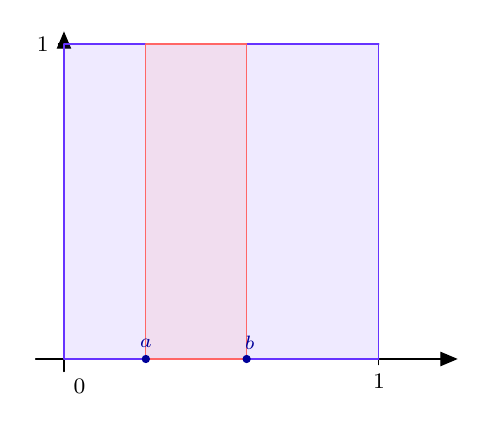
\begin{tikzpicture}[line cap=round,line join=round,>=triangle 45,x=4.0cm,y=4.0cm]
        \draw[->,color=black] (-0.09,0) -- (1.25,0);
        \foreach \x in {,1}
        \draw[shift={(\x,0)},color=black] (0pt,2pt) -- (0pt,-2pt) node[below] {\footnotesize $\x$};
        \draw[->,color=black] (0,-0.04) -- (0,1.04);
        \foreach \y in {,1}
        \draw[shift={(0,\y)},color=black] (2pt,0pt) -- (-2pt,0pt) node[left] {\footnotesize $\y$};
        \draw[color=black] (0pt,-10pt) node[right] {\footnotesize $0$};
        \clip(-0.09,-0.04) rectangle (1.25,1.04);
        \fill[color=wwttff,fill=wwttff,fill opacity=0.1] (0,0) -- (0,1) -- (1,1) -- (1,0) -- cycle;
        \fill[color=ffwwww,fill=ffwwww,fill opacity=0.1] (0.26,1) -- (0.58,1) -- (0.58,0) -- (0.26,0) -- cycle;
        \draw [color=wwttff] (0,0)-- (0,1);
        \draw [color=wwttff] (0,1)-- (1,1);
        \draw [color=wwttff] (1,1)-- (1,0);
        \draw [color=wwttff] (1,0)-- (0,0);
        \draw [color=ffwwww] (0.26,1)-- (0.58,1);
        \draw [color=ffwwww] (0.58,1)-- (0.58,0);
        \draw [color=ffwwww] (0.58,0)-- (0.26,0);
        \draw [color=ffwwww] (0.26,0)-- (0.26,1);
        \begin{scriptsize}
            \fill [color=qqqqzz] (0.26,0) circle (1.5pt);
            \draw[color=qqqqzz] (0.26,0.05) node {$a$};
            \fill [color=qqqqzz] (0.58,0) circle (1.5pt);
            \draw[color=qqqqzz] (0.59,0.05) node {$b$};
        \end{scriptsize}
    \end{tikzpicture}
    &&\definecolor{wwwwww}{rgb}{0.4,0.4,0.4}
    \definecolor{qqqqcc}{rgb}{0,0,0.8}
    \definecolor{qqqqff}{rgb}{0,0,1}
    \definecolor{qqqqzz}{rgb}{0,0,0.6}
    \definecolor{ffqqtt}{rgb}{1,0,0.2}
    \definecolor{zzttqq}{rgb}{0.6,0.2,0}
    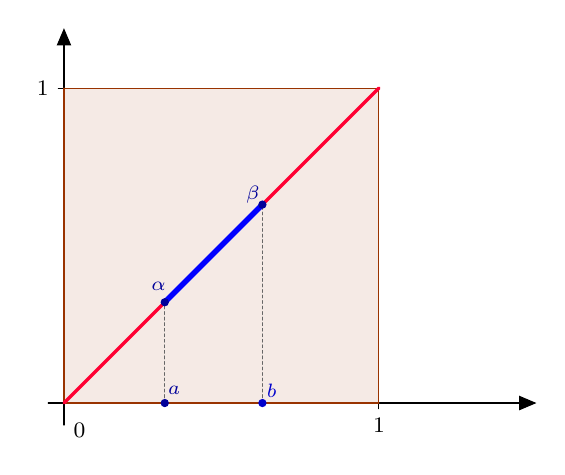
\begin{tikzpicture}[line cap=round,line join=round,>=triangle 45,x=4.0cm,y=4.0cm]
        \draw[->,color=black] (-0.05,0) -- (1.5,0);
        \foreach \x in {,1}
        \draw[shift={(\x,0)},color=black] (0pt,2pt) -- (0pt,-2pt) node[below] {\footnotesize $\x$};
        \draw[->,color=black] (0,-0.07) -- (0,1.19);
        \foreach \y in {,1}
        \draw[shift={(0,\y)},color=black] (2pt,0pt) -- (-2pt,0pt) node[left] {\footnotesize $\y$};
        \draw[color=black] (0pt,-10pt) node[right] {\footnotesize $0$};
        \clip(-0.05,-0.07) rectangle (1.5,1.19);
        \fill[color=zzttqq,fill=zzttqq,fill opacity=0.1] (0,0) -- (0,1) -- (1,1) -- (1,0) -- cycle;
        \draw [color=zzttqq] (0,0)-- (0,1);
        \draw [color=zzttqq] (0,1)-- (1,1);
        \draw [color=zzttqq] (1,1)-- (1,0);
        \draw [color=zzttqq] (1,0)-- (0,0);
        \draw [line width=1.2pt,color=ffqqtt] (0,0)-- (1,1);
        \draw [line width=2pt,color=qqqqff] (0.32,0.32)-- (0.63,0.63);
        \draw [dash pattern=on 1pt off 1pt,color=wwwwww] (0.32,0)-- (0.32,0.32);
        \draw [dash pattern=on 1pt off 1pt,color=wwwwww] (0.63,0)-- (0.63,0.63);
        \begin{scriptsize}
            \fill [color=qqqqzz] (0.32,0.32) circle (1.5pt);
            \draw[color=qqqqzz] (0.30,0.37) node {$\alpha$};
            \fill [color=qqqqzz] (0.63,0.63) circle (1.5pt);
            \draw[color=qqqqzz] (0.60,0.66) node {$\beta$};
            \fill [color=qqqqzz] (0.32,0) circle (1.5pt);
            \draw[color=qqqqzz] (0.35,0.04) node {$a$};
            \fill [color=qqqqcc] (0.63,0) circle (1.5pt);
            \draw[color=qqqqcc] (0.66,0.04) node {$b$};
        \end{scriptsize}
    \end{tikzpicture}\\
    &\text{a) Первый случай} &&\text{б) Второй случай}\\
    &\mu_{X, Y}(B) = S_B &&\mu_{X, Y} = P((X, Y) \in [\alpha, \beta]) = \frac{\beta-\alpha}{\sqrt{2}}\\
    &P(X \in [a, b]) = b - a &&P(X \in [a, b]) = \frac{(b - a)\sqrt{2}}{\sqrt{2}}=b - a\\
    &P(Y \in [a, b]) = b - a &&P(Y \in [a, b]) = \frac{(b - a)\sqrt{2}}{\sqrt{2}}=b - a\\
\end{align*}
В этих двух случаях случайные величины $X, Y$ имеют одинаковое распределение, однако их совместные распределения
отличаются. Так, например, для первого случая вероятность выбора точки из любого множества, непересекающегося с диагональю
не равна нулю, однако это не верно для второго случая. На основании этих случаев мы можем сделать вывод, что
если известно распределение каждой из случайных величин, то даже тогда мы не можем узнать их совместное распределение.

\subsection{Абсолютно непрерывные случайные распределения.}
Пусть $(\Omega, \mathcal{A}, P)$ --- вероятностое пространство, в $X, Y$ --- случайные величины на нём.
\begin{definition}
    Совместное распределение случайных величин $X, Y$ называется \it{абсолютно непрерывным}, если существует
    такая интегрируемая и неотрицательная функция $\rho_{X, Y}(t, s)$, что
    \[
        F_{X, Y}(t, s) = \iint\limits_{(-\infty, t] \times (-\infty, s]} \rho_{X, Y}(t, s) dtds
    \]
    Функция $\rho_{X, Y}$ называется \it{плотностью} совместного распределения случайных величин $X, Y$.
\end{definition}
Можно показать, что
\[
    P(a < X \leq b, c < Y \leq d) = \mu_{X, Y}((a, b] \times (c, d]) =
    \iint\limits_{(a, b] \times (c, d]} \rho_{X, Y}(t, s) dtds
\]
Кроме того в каждой точке непрерывности функции $\rho_{X, Y}$ выполнено равенство
\[
    \frac{\partial^2}{\partial t\partial s} F_{X, Y}(t, s) = \rho_{X, Y}(t, s)
\]
Если известна плотность совместного распределения $\rho_{X, Y}$, то можно найти плотность каждой из компонент:
\begin{align*}
    &F_X(t) = P(X \leq y, Y \in \RR) = \int\limits_{-\infty}^{t} dx \int\limits_{-\infty}^{\infty} \rho_{X, Y}(x, y) dy \implies\\
    &\implies F_X'(t) = \rho_X(t) = \int\limits_{-\infty}^{\infty} \rho_{X, Y}(x, y) dy
\end{align*}
Заметим однако, что совместное распределение может не иметь плотности вообще.

На самом деле можно доказать, что
\[
    \mu_{X, Y} = P((X, Y) \in B) = \iint\limits_{B} \rho_{X, Y} (t, s) dtds
\]
\begin{theorem}
    Пусть распределение $X, Y$ задано плотностью $\rho_{X, Y}$. Рассмотрим случайные величины $\xi = f(X, Y),
    \eta = g(X, Y)$. Пусть отображение $\phi \colon (x, y) \to
    \left( \underbrace{f(x, y)}_{u}, \underbrace{g(x, y)}_{v} \right)$ биективно,
    $\phi, \phi^{-1}$ --- непрерывно дифференцируемы, и $\det J_\phi \neq 0$. Тогда
    $\rho_{\xi, \eta} = \rho_{X, Y} \left( \phi^{-1}(u, v) \right) \cdot \left| \det J_\phi^{-1}(\phi^{-1}(u, v)) \right|$.
\end{theorem}
\begin{proof}
    Свойство матрицы Якоби: матрица Якоби обратной функции, взятая в точке $(u, v)$ равна обратной матрице Якоби функции,
    взятая в точке $f^{-1}(u, v)$. Т.е. пусть $\psi$ --- функция, тогда
    \[
        J_{\psi^{-1}}(u, v) = \left( J_{\psi}^{-1} (\psi^{-1}(u, v)) \right)
    \]
    Заметим, что
    \[
        P\left( (\xi, \eta) \in B \right) = P\left( (X, Y) \in \phi^{-1}(B) \right) =
        \iint\limits_{\phi^{-1}(B)} \rho_{X, Y}(x, y) dxdy
    \]
    Сделаем замену: $(u, v) = \phi(x, y) \implies (x, y) = \phi^{-1}(u, v)$. Тогда
    \[
        \iint\limits_{\phi^{-1}(B)} \rho_{X, Y}(x, y) dxdy =
        \iint\limits_{B} \rho_{X, Y}(\phi^{-1}(u, v)) \cdot \left|\det\left( J_{\phi}^{-1} (\phi^{-1}(u, v)) \right)\right| dudv
    \]
    Таким образом мы получили, что
    \[
        P\left( (\xi, \eta) \in B \right) =
        \iint\limits_{B} \rho_{X, Y}(\phi^{-1}(u, v)) \cdot \left|\det\left( J_{\phi}^{-1} (\phi^{-1}(u, v)) \right)\right| dudv
        \iff
        \rho_{\xi, \eta} = \rho_{X, Y}(\phi^{-1}(u, v)) \cdot \left|\det\left( J_{\phi}^{-1} (\phi^{-1}(u, v)) \right)\right|
    \]
\end{proof}

\subsection{Многомерное равномерное распределение.}
Пусть $(\Omega, \mathcal{A}, P)$ --- вероятностное пространство, а $\xi_1, \xi_2, \ldots, \xi_n$ --- случайные
величины на нём.
\begin{definition}
    Вектор $(\xi_1, \xi_2, \ldots, \xi_n)$ имеет \it{равномерное распределение} на множестве $B \subset \Omega$,
    если
    \[
        P\left( (\xi_1, \xi_2, \ldots, \xi_n) \in B \right) = \frac{\vol(B)}{\vol(\Omega)} =
        \idotsint\limits_{B} \frac{1}{\vol(\Omega)} dx_1 dx_2 \ldots dx_n
    \]
    Иначе говоря, вектор равномерно распределён, если его распределение задано плотностью
    \[
        \rho(x_1, x_2, \ldots, x_n) =
        \begin{cases}
            \frac{1}{\vol(\Omega)} & (x_1, x_2, \ldots, x_n) \in B\\
            0 & (x_1, x_2, \ldots, x_n) \notin B
        \end{cases}
    \]
    Под $\vol$ везде подразумевается \it{разумная функция}, отвечающая нашему понимаю измерения объёма в $n$-мерном случае.
    В одномерном случае эта функция эквивалентна мере Лебега, в двумерном --- площади, в трёхмерном --- объёму.
\end{definition}

Пусть теперь множество $B$ --- произвольное. Тогда вектор $(\xi_1, \xi_2, \ldots, \xi_n)$ равномерно
на нём распределён, если
\[
    P\left( (\xi_1, \xi_2, \ldots, \xi_n) \in B \right) = \frac{\vol(B \cap \Omega)}{\vol(\Omega)} =
    \idotsint\limits_{B} \frac{1}{\vol(\Omega)} \cdot I_{\Omega}(x_1, x_2, \ldots, x_n) dx_1 dx_2 \ldots dx_n
\]
где $I_{\Omega}(x_1, x_2, \ldots, x_n)$ возвращает $1$, если $(x_1, x_2, \ldots, x_n) \in \Omega$ (индикатор).
Иначе говоря, вектор равномерно распределён на произвольном множестве $B$, если его распределение задано плотностью:
\[
    \[
        \rho(x_1, x_2, \ldots, x_n) =
        \begin{cases}
            \frac{1}{\vol(\Omega)} & (x_1, x_2, \ldots, x_n) \in B \cap \Omega\\
            0 & (x_1, x_2, \ldots, x_n) \notin B \cap \Omega
        \end{cases}
    \]
\]

\subsection{Независимые случайные величины.}
Пусть $(\Omega, \mathcal{A}, P)$ --- вероятностное пространство, а $X, Y$ --- случайные
величины на нём.
\begin{definition}
    Случайные величины $X, Y$ называются \it{независимыми} тогда и только тогда, когда
    \[
        F_{X, Y}(t, s) = F_X(t)F_Y(s)
    \]
\end{definition}
\begin{proposal}
    Случайные величины $X, Y$ независимы тогда и только тогда, когда для произвольных $A, B \in \mathcal{B}(\RR)$
    выполнено
    \[
        P(X \in A, Y \in B) = P(X \in A) \cdot P(Y \in B)
    \]
\end{proposal}
\begin{proof}
    ~\\
    $\Leftarrow \colon$ Очевидно по определению (лучи --- Борелевские множества).\\
    $\Rightarrow \colon$ Пусть $B$ --- луч, если $P(Y \in B) = 0$, тогда с левой стороны $0$, и справой тоже $0$,
    т.к. $\{X \in A, Y \in B\} \subset \{Y \in B\}$. Далее считаем, что $P(Y \in B) \neq 0$. Тогда положим
    $Q(A) = \frac{P(X \in A, Y \in B)}{P(Y \in B)}$. Нетрудно понять, что
    $Q\left( \bigcup_{k = 1}^{\infty} A_k \right) = \sum\limits_{k = 1}^{\infty} Q(A_k)$. Отсюда следует, что
    $Q$ --- счётно-аддитивная вероятностная мера на $\mathcal{B}(\RR)$. Известно, что $Q(A) = \mu_X(A)$, когда
    $A$ --- луч. Тогда мы имеем: $Q$ --- счётно-аддитивная мера на алгебре лучей. По теореме Лебега:
    существует единственная мера, которая совпадает с $Q$ на этой алгебре, и продолжает её на $\sigma$-алгебру,
    порождённую этой алгеброй. \href{https://raw.githubusercontent.com/johanDDC/My_TeXs/5981fbe92fbd8dfae37ea2c29fbf204a942d0d09/pdf/Lebeg/Lebeg.pdf}{В конспекте по теории меры Лебега} (пункт 2.3)
    доказывалось, что $\sigma$-алгебра, порождённая алгеброй лучей совпадает с $\mathcal{B}(\RR)$. Значит,
    $\mu_X$ --- то самое, единственное продолжение $Q$ на любое Борелевское множество.

    Пусть теперь $A \in \mathcal{B}$ --- фиксированное Борелевское множество, и $P(X \in A) \neq 0$ (понятно, что
    если $P(X \in A) = 0$, то всё выполнено). Рассмотрим теперь вероятностную меру
    \[
        Q'(B) = \frac{P(X \in A, Y \in B)}{P(X \in A)}
    \]
    По аналогии с $Q(A), Q'(B)$ счётно-аддитивна. И $Q'(B) = \mu_Y(B)$, если $B$ --- луч. Тогда, по аналогии с
    $Q(A)$ всё снова выполнено для любого Борелевского $B$.
\end{proof}
\begin{comment}
    Обоснование счётной-аддитивности $Q(A)$:\\
    Заметим, что $\{X \in A, Y \in B\} = \{X \in A\} \cap \{Y \in B\}$. Тогда
    \begin{align*}
        Q\left( \bigcup_{k = 1}^{\infty} A_k \right) &=
        \frac{P\left(\left\{
        X \in \bigcup\limits_{k = 1}^{\infty} A_k, Y \in B
        \right\}\right)}{P(Y \in B)} =
        \frac{P\left(\left\{
        X \in \bigcup\limits_{k = 1}^{\infty} A_k\right\} \cap \left\{ Y \in B
        \right\}\right)}{P(Y \in B)} =
        \frac{P\left( \bigcup\limits_{k = 1}^{\infty}
        \{X \in A_k\} \cap \{ Y \in B
        \}\right)}{P(Y \in B)} =\\
        &= \sum\limits_{k = 1}^{\infty} Q(A_k)
    \end{align*}
    В последнем переходе использована счётная аддитивность $P$.
\end{comment}
\begin{definition}
    Функция $f \colon \RR \to \RR$ называется \it{Борелевской}, если $f^{-1}((-\infty, t]) \in \mathcal{B}(\RR)$
    для всякого действительного $t$.
\end{definition}
\begin{corollary}
    Если $f, g$ --- Борелевские функции, а $X, Y$ --- независимые случайные величины на вероятностном пространстве,
    то случайные величины $f(X), g(Y)$ также независимы.\\
    Действительно
    \[
        P(f(X) \in A, g(Y) \in B) = P(X \in f^{-1}(A), Y \in g^{-1}(B)) =
        P(X \in f^{-1}(A)) \cdot P(Y \in g^{-1}(B)) = P(f(X) \in A) \cdot P(g(Y) \in B)
    \]
\end{corollary}
\begin{proposal}
    Пусть распределения $X$ и $Y$ заданы плотностями. Тогда $X$ и $Y$ независимы тогда и только тогда, когда
    плотность их совместного распределения имеет вид
    \[
        \rho_{X, Y}(t, s) = \rho_X(t)\rho_Y(s)
    \]
\end{proposal}
\begin{proof}
    ~\\
    $\Rightarrow \colon$
    \[
        F_{X, Y} (x, y) = F_X(x)F_Y(y) = \int\limits_{-\infty}^{x} \rho_X(t)dt
        \int\limits_{-\infty}^{y} \rho_Y(s)ds = \iint\limits_{(-\infty, x] \times (-\infty, y]}
        \underbrace{\rho_X(t)\rho_Y}_{\rho_{X, Y}(t, s)}(s)dtds
    \]
    $\Leftarrow \colon$
    \[
        F_{X, Y} (x, y) = \iint\limits_{(-\infty, x] \times (-\infty, y]}
        \rho_{X, Y}(t, s)dtds = \iint\limits_{(-\infty, x] \times (-\infty, y]}
        \rho_X(t)\rho_Y(s)dtds = \int\limits_{-\infty}^{x} \rho_X(t)dt
        \int\limits_{-\infty}^{y} \rho_Y(s)ds = F_X(x)F_Y(y)
    \]
\end{proof}
\begin{corollary}[Формула свёртки]
    Пусть $X, Y$ независимы, и их распределения заданы плотностями. Тогда распределение
    $Z = X + Y$ задано плотностью
    \[
        \rho_Z(z) = \int\limits_{-\infty}^{\infty} \rho_X(t)\rho_Y(z - t) dt
    \]
\end{corollary}
\begin{proof}
    По определению функции распределения:
    \[
        F_Z(t) = P(X + Y \leq t) = \iint\limits_{x + y \leq t} \rho_X(x)\rho_Y(y) dxdy
    \]
    Сделаем замену: $u = x + y, v = x$. Тогда
    \[
        \begin{cases}
            u = x + y\\
            v = x
        \end{cases}
        \iff
        \begin{cases}
            x = v\\
            y = u - v
        \end{cases},
        ~~~
        \det J =
        \begin{vmatrix}
            \frac{\partial x}{\partial u} & \frac{\partial x}{\partial v}\\
            \frac{\partial y}{\partial u} & \frac{\partial y}{\partial v}
        \end{vmatrix}
        =
        \begin{vmatrix}
            0 & 1\\
            1 & -1
        \end{vmatrix}
        = -1
    \]
    И, подставляя замену в интеграл имеем
    \[
        F_Z(t) = \iint\limits_{x + y \leq t} \rho_X(x)\rho_Y(y) dxdy
        = \iint\limits_{u \leq t} \rho_X(v)\rho_Y(u - v) dudv
        = \int\limits_{-\infty}^{t} du \int\limits_{-\infty}^{\infty} \rho_X(v)\rho_Y(u - v) dv
    \]
    Отсюда $\rho_Z(u) = \int\limits_{-\infty}^{\infty} \rho_X(v)\rho_Y(u - v) dv$.
\end{proof}

\subsection{Математическое ожидание в общем случае: ограниченные случайные величины.}
\begin{definition}
    Пусть $X$ --- ограниченная случайная величина (т.е. существует $b > 0 \colon \forall w \in \Omega \implies |X(w)| < b$). Тогда
    её \it{математическим ожиданием} называется $\lim\limits_{n \to \infty} \EE(X_n)$, где $X_n$ --- последовательность произвольных
    случайных величин с конечным числом значений, равномерно сходящаяся к $X$.
\end{definition}
Проверим корректность определения, а именно проверим, что
\begin{lemma}
    Для произвольной ограниченной случайной величины $X$ найдётся последовательность случайных величин с конечным числом значений
    $X_n$, равномерно сходящаяся к $X$.
\end{lemma}
\begin{proof}
    Ограниченность случайной величины $X$ означает что $\exists b > 0 \colon \forall w \in \Omega \implies |X(w)| < b$. Это
    равносильно тому что $X$ принимает значения из интервала $(-b, b)$. Пройдёмся по этому интервалу, и разобьём его на сколько-то
    дизъюнктных полуинтервалов длины $\frac{2b}{n}$. Тогда $k$-ый полуинтервал будет иметь вид:
    $\left[-b + (k - 1)\frac{2b}{n}, -b + k\frac{2b}{n}\right)$. Обозначим $k$-ый полуинтервал за $J_k$. Положим случайную величину
    $X_n$ --- для произвольной $w \in \Omega$ выполняется, что $X(w)$ попало в $k$-ый полуинтервал. Тогда
    \[
        X_n(w) = \sum\limits_{k = 1}^{n} \left( -b + (k - 1)\frac{2b}{n} \right) \cdot I_{X(w) \in J_k}
    \]
    где $I_{X(w) \in J_k}$ --- индикатор соответствующего события. Таким образом $X_n$ принимает не более чем $n$ значений.
    Выберем теперь произвольную $w_0 \in \Omega$. Известно, что $X(w_0)$ попдает в какой-то полуинтервал, пусть она попала в
    $J_k$. Тогда $X_n(w_0) = -b + (k - 1)\frac{2b}{n}$, т.е. это в точности начало $k$-ого полуинтервала. Оценим теперь
    $|X_n(w_0) - X(w_0)|$. Заметим, что $X_n(w_0)$, как уже отмечалось выше, конец $k$-ого полуинтервала, а $X(w)$ --- какая-то
    точка из этого полуинтервала. Тогда модуль разницы между ними мы можем оценить сверху длиной всего полуинтервала:
    \[
        |X_n(w_0) - X(w_0)| \leq \left| J_k \right| = \frac{2b}{n}
    \]
    Получили, что в каждой точке разница случайных величин не превосходит $\frac{2b}{n}$. Ну тогда выполняется, что
    \[
        \sup|X_n(w) - X(w)| \leq \frac{2b}{n} \to 0
    \]
    А это в точности определение равномерной сходимости.
\end{proof}
\begin{comment}
    Если не появилось понимания того что произошло, очень рекомендую посмотреть это доказательство в
    \href{https://drive.google.com/file/d/1JuT1me8rnYAElmNJomesxIowCqU3LlEv/view}{лекции}, там оно получилось
    на редкость удачное. Таймкод: $26:22$.
\end{comment}
Итак, мы теперь знаем, что такие последовательности найдутся. Для полного счастья и уверенности в корректности определения
нам теперь нужно понять, что предел их матожиданий существует.
\begin{proposal}
    Для произвольной ограниченной случайной величины $X$, и для произвольной последовательности случайных величин, имеющих
    конечное число значений $X_n$, равномерно сходящейся к $X$ существует предел $\lim\limits_{n \to \infty} \EE(X_n)$.
    Более того, для другой такой последовательности $Y_n$, также равномерно сходящейся к $X$ выполнено $\lim \EE(X_n) = \lim \EE(Y_n$.
\end{proposal}
\begin{proof}
    Заметим, что
    \[
        |\EE(X_n) - \EE(X_k)| = \EE(|X_n - X_k|) \leq
        \sup_{w \in \Omega}|X_n(w) - X_k(w)|
    \]
    Отсюда следует фундаментальность последовательности $\{\EE(X_n)\}$, а значит её предел существует.\\
    Пусть теперь $Y_n$ --- другая последовательность случайных величин с конечным числом значений, равномерно сходящаяся к
    $X$. Составим последовательность $Z_n$ --- по следующему правилу: на чётных местах расположим элементы последовательности
    $X_n$, на нечётных $Y_n$. Тогда $Z_n$ будет обладать теми же свойствами, и, в частности, равномерно сходиться к $X$.
    Тогда уже доказали, что существует предел $\{\EE(Z_n)\}$, и тогда $\lim \EE(Y_n) = \lim \EE(X_n)$ как пределы
    подпоследовательностей сходящейся последовательности.
\end{proof}
Переходим к свойствам вновь определённого матожидания:
\begin{proposal}
    Для произвольных ограниченных случайных величин $X, Y$ выполнены свойства матожидания:
    \begin{enumerate}
        \item $\EE(aX + bY) = a\EE(X) + b\EE(Y)$.
        \item Если $X \geq 0$ почти наверное, то $\EE(X) \geq 0$, в частности если $X \geq Y$, то $\EE(X) \geq \EE(Y)$.
    \end{enumerate}
\end{proposal}
\begin{proof}
    ~\\
    1) Если $X_n, Y_n$ --- принимают конечное число значений, и $X_n \rightrightarrows X, Y_n \rightrightarrows Y$, то
    $aX_n + bY_n \rightrightarrows aX + bY$, и $\EE(aX + bY) = \lim \EE(aX_n + bY_n) = a\lim \EE(X_n) + b\lim \EE(Y_n) =
    a\EE(X) + b\EE(Y)$.\\
    2) Пусть $\forall w \in \Omega \implies X(w) \geq 0$, а $X_n$ --- принимает конечное число значений,
    и $X_n \rightrightarrows \sqrt{X}$. Тогда $X_n^2 \rightrightarrows X$, и $\EE(X) = \lim \EE(X_n^2) \geq 0$.\\
    Вторая часть утверждения: пусть для произвольного $X \geq 0$ почти наверное выполнено
    $\EE(X) = \EE(X \cdot I_{X \geq 0}) + \EE(X \cdot I_{X < 0})$. Известно, что при $X < 0, -X$ --- неотрицательая
    случайная величина. Тогда для неё выполнено $\EE(-X \cdot I_{X < 0}) \geq 0$. В силу ограниченности $X$:
    $\EE((b - -X) \cdot I_{X < 0}) = \EE((b + X) \cdot I_{X < 0}) \geq 0$. Теперь следим за руками:
    \begin{align*}
        \EE((b + X) \cdot I_{X < 0}) \geq 0
        &\iff
        \EE(b \cdot I_{X < 0}) + \EE(X \cdot I_{X < 0}) \geq 0
        \iff
        -\EE(X \cdot I_{X < 0}) \leq b\underbrace{\EE(I_{X < 0})}_{P(X < 0)}
        \iff\\
        &\iff
        0 \leq \EE(-X \cdot I_{X < 0}) \leq b \cdot P(X < 0) = 0
    \end{align*}
    Cоответственно при $X \geq Y$ почти наверное имеем $X - Y \geq 0$ почти наверное, и тогда
    $\EE(X - Y) \geq 0 \iff \EE(X) \geq \EE(Y)$.
\end{proof}
\subsection{Математическое ожидание в общем случае: неотрицательные случайные величины.}
\begin{definition}
    Пусть $\forall w \in \Omega \implies X(w) \geq 0$ --- неотрицательная случайная величина. Её
    \it{математическим ожиданием} называется конечное число
    \[
        \EE(X) = \sup \{\EE(U) \colon 0 \leq U \leq X, U \text{ --- ограниченная }\}
    \]
\end{definition}
\begin{proposal}
    Для неотрицательных случайных величин $X, Y$ выполнены следующие свойства матожидания:
    \begin{enumerate}
        \item $\EE(aX + bY) = a\EE(X) + b\EE(Y)$, при $a, b \geq 0$.
        \item Если $X \geq Y \geq 0$, то $\EE(X) \geq \EE(Y)$. В частности, если $\EE(X)$ --- конечно, то и $\EE(Y)$ ---
        конечно.
        \item Если $X = 0$ почти наверное, то $\EE(X) = 0$.
    \end{enumerate}
\end{proposal}
\begin{proof} ~\\
    1) Ясно, что доказать для $a = b = 1$ достаточно. Если $0 \leq U \leq X$, и $0 \leq V \leq Y$, то
    $U + V \leq X + Y \iff \EE(X) + \EE(Y) \leq \EE(X + Y)$.\\
    В другую сторону: пусть $0 \leq Z \leq X + Y$, $U = \min(X, Z)$, $V = Z - U$. Тогда $0 \leq U \leq X,
    V = (Z - X) \cdot I_{X < Z} \leq X + Y - X = Y$. Тогда $\EE(Z) = \EE(U + V) \leq \EE(X) + \EE(Y) \implies
    \EE(X + Y) \leq \EE(X) + \EE(Y)$.\\
    Все введённые случайные величины считались ограниченными.\\
    2) Очевидно.\\
    3) Пусть $0 \leq U \leq X$ --- ограниченная случайная величина, и $X = 0$ почти наверное. Тогда $U = 0$ почти наверное и
    \[
        \EE(U) = \EE(U \cdot I_{U \neq 0}) \leq \EE(\sup U \cdot I_{U \neq 0}) = \sup U \cdot P(U \neq 0) = 0
    \]
\end{proof}
\subsection{Математическое ожидание в общем случае: реально общий случай.}
\begin{designation}
    В этой главе мы будем применять следующие два обозначения:
    \begin{enumerate}
        \item $X^+ = \max\{X, 0\} \geq 0$.
        \item $X^- = \max\{-X, 0\} \geq 0$.
    \end{enumerate}
    При этом заметим, что произвольная случайная величина $X$ обладает свойством $X = X^+ - X^-$.
\end{designation}
Пусть $X^+, X^-$ обладают конечным матожиданием.
\begin{definition}
    \it{Математическим ожиданием} произвольной случайной величины $X$ называется число
    \[
        \EE(X) = \EE(X^+) - \EE(X^-)
    \]
\end{definition}
Проверим корректность определения в следующем смысле: если есть случайные величины $U \geq 0, V \geq 0$, и $X$ через них выражается
как $X = U - V$, то с одной стороны $X$ выражается через них, а с другой стороны $X = X^+ - X^-$, и в этой ситуации нам бы
хотелось чтобы выполнялось следующее:
\[
    \begin{cases}
        X = U - V\\
        X = X^+ - X^-
    \end{cases}
    \implies
    \EE(U) - \EE(V) = \EE(X^+) - \EE(X^-)
\]
Ну и действительно имеем $X = U - V = X^+ - X^- \iff U + X^- = X^+ + V \implies \EE(U + X^-) = \EE(X^+ + V)$. В силу неотрицательности
вообще всех случайных величин в этом равенстве имеем $\EE(U) + \EE(X^-) = \EE(X^+) + \EE(V)$. Переносим в правильную сторону
и получаем то что хотели.
\begin{proposal}
    Для произвольных случайных величин $X, Y$ выполнены следующие свойства матожидания:
    \begin{enumerate}
        \item $\EE(aX + bY) = a\EE(X) + b\EE(Y)$.
        \item Если $X \geq 0$ почти наверное, то $\EE(X) \geq 0$, и если $X \geq Y$, то $\EE(X) \geq \EE(Y)$.
        \item Если $X \geq 0$ почти наверное, и $\EE(X) = 0$, то $X = 0$ почти наверное.
        \item $|\EE(X)| \leq \EE(|X|)$.
    \end{enumerate}
\end{proposal}
\begin{proof} ~\\
    1) Ясно, что достаточно доказать для случая $a, b \geq 0$. Известно, что $aX + bY = (aX^+ + bY^+) - (aX^- + bY^-)$,
    причём каждое из слагаемых --- неотрицательная случайная величина. Имеем:
    \begin{align*}
        \EE(aX + bY) &= \EE(aX^+ + bY^+) - \EE(aX^- + bY^-) = a\EE(X^+) + b\EE(Y^+) - a\EE(X^-) - b\EE(Y^-) =\\
        &=a\left( \EE(X^+) - \EE(X^-) \right) + b\left( \EE(Y^+) - \EE(Y^-) \right) = a\EE(X) + b\EE(Y)
    \end{align*}
    2) $X \geq 0$ почти наверное $\implies X^- = 0$ почти наверное $\implies \EE(X) = \EE(X^+) \geq 0$.\\
    3)
    \[
        P(X > 0) = P\left( \bigcup_{k = 1}^{\infty} X \geq \frac{1}{k} \right) =
        \sum\limits_{k = 1}^{\infty} P\left( X \geq \frac{1}{k} \right)
    \]
    Рассмотрим случайную величину $\frac{1}{k} \cdot I_{X \geq \frac{1}{k}}$. Понятно, что она не превосходит $X$. Тогда
    с одной стороны $\EE\left( \frac{1}{k} \cdot I_{X \geq \frac{1}{k}} \right) \leq \EE(X) = 0$, а с другой стороны
    $\EE\left( \frac{1}{k} \cdot I_{X \geq \frac{1}{k}} \right) = \frac{1}{k}P\left( X \geq \frac{1}{k} \right)$.
    Тогда $\frac{1}{k}P\left( X \geq \frac{1}{k} \right) = 0 \iff P\left( X \geq \frac{1}{k} \right) = 0$. Из равенства выше
    получаем требуемое.\\
    4) Аналогично дискретному случаю: понятно, что $-|X| \leq X \leq |X|$. Теперь по монотонности навешиваем матожидание и
    получаем требуемое.
\end{proof}
\subsection{Матожидание функции от случайной величины с абсолютно непрерывным распределением.}
Пусть $(\Omega, \mathcal{A}, P)$ --- вероятностное пространство.
\begin{lemma}
    Пусть $X$ --- произвольная неотрицательная случайная величина, $A_n \subset A_{n + 1}, A_n \in \mathcal{A}$, причём $A_n$
    в объединении дают $\Omega$. Тогда $\EE(X) < \infty \iff \sup_{n}\EE(X \cdot I_{A_n}) = M < \infty$. Более того:
    $\EE(X) = \lim\EE(X \cdot I_{A_n}) = M$.
\end{lemma}
\begin{proof}
    Пусть $0 \leq U \leq X$ --- произвольная ограниченная случайная величина. Тогда
    $\EE(U \cdot I_{A_n}) \leq \EE(X \cdot I_{A_n}) \leq M$. Известно, что
    $\EE(U) = \EE(U \cdot I_{A_n}) + \EE(U \cdot I_{\Omega \setminus A_n})$, при этом
    $\EE(U \cdot I_{\Omega \setminus A_n}) \leq \sup U \cdot P(\Omega \setminus A_n)$. Последняя вероятность
    стремится к нулю из-за вложенности множеств $A_n$. Тогда $\EE(U) = \lim\limits_{n \to \infty} \EE(U \cdot I_{A_n})$.
    Но т.к. по самой первой оценке при каждом $n$ $U \cdot I_{A_n} \leq M$, то предел их ожиданий так же не превосходит $M$. А
    также ожидание супремума не превосходит $M$, но рассматривать супремум $U$ всё равно что рассматривать $X$. Отсюда
    $\EE(X) \leq M$.\\
    В другую сторону: пусть теперь $\EE(X)$ --- конечно. Тогда очевидно, что $X \geq X \cdot I_{A_n}$. Отсюда по монотонности
    матожидания $\EE(X) \geq \EE(X \cdot I_{A_n})$, а значит это выполнено и для супремума.
\end{proof}
\begin{proposal}
    Пусть $X$ --- произвольная случайная величина, распределение которой задано плотностью $\rho_X$ (т.е. это абсолютно непрерывная
    случайная величина). Пусть задана непрерывная функция $f$. Тогда матожидание $\EE(f(X))$ существует тогда и только тогда, когда
    сходится несобственный интеграл
    \[
        \int\limits_{-\infty}^{+\infty} |f(t)|\rho_X(t)dt
    \]
    Более того, в случае сходимости
    \[
        \EE(f(X)) = \int\limits_{-\infty}^{+\infty} f(t)\rho_X(t)dt
    \]
\end{proposal}
\begin{proof}
    Достаточно доказать для $f \geq 0$. Иначе проводим аналогичные рассуждения для $f(X) =f^+(X) - f^-(X)$.
    Рассмотрим ограниченный отрезок $[-R, R]$. Разбив его на $N$ подотрезков мы можем приблизить функцию $f$
    ступенчатыми функциями $g_n$, которые имеют вид $g_n = \sum\limits_{j = 1}^{N_n} c_j \cdot I_{[a_j, b_j]}$. Причём эти
    ступенчатые функции будут равномерно сходиться к $f$. Тогда справедлива следующая оценка:
    \begin{align*}
        \left| \EE(f(t) \cdot I_{X \in [-R, R]}) - \EE(g_n(t)) \right| &=
        \left| \EE \left( (f(t) - g_n(t)) \cdot I_{X \in [-R, R]} \right) \right| \leq
        \EE \left( \left| f(x) - g_n(x) \right| \cdot I_{X \in [-R, R]} \right) \leq\\
        &\leq \sup_{[-R, R]} |f(t) - g_n(t)|
    \end{align*}
    И такая же оценка справедлива для интегралов:
    \begin{align*}
        \left|\int\limits_{-R}^{R} f(t)\rho_X(t)dt - \int\limits_{-R}^{R} g_n(t)\rho_X(t)dt\right|
        = \int\limits_{-R}^{R} |f(t) - g_n(t)|\rho_X(t)dt \leq \sup_{[-R, R]} |f - g_n| \cdot \underbrace{\int\limits_{-R}^{R} \rho_X(t)dt}_{1}
    \end{align*}
    В силу равномерной сходимости: $g_n \rightrightarrows f \iff \sup|f - g_n| \to 0$. Кроме того можно замеить, что
    \[
        \EE(g_n(X)) = \sum\limits_{j = 1}^{N_n}c_j \EE(I_{X \in [a_j, b_j]}) =
        \sum\limits_{j = 1}^{N_n}c_j P(X \in [a_j, b_j]) =
        \sum\limits_{j = 1}^{N_n}c_j \int\limits_{a_j}^{b_j} \rho_X(t)dt =
        \int\limits_{-R}^R g_n(t)\rho_X(t)dt
    \]
    Тогда из всех предыдущих оценок следует, что
    \[
        \EE(f(X) \cdot I_{X \in [-R, R]}) = \int\limits_{-R}^R f(t)\rho_X(t)dt
    \]
    Устремляя $R \to \infty$ Получаем утверждение.
\end{proof}
\begin{comment}
    На мой взгляд как-то скомканно, можно посмотреть в 
    \href{https://drive.google.com/file/d/1KgHK_Z_ms3UNI4WAbLlRuI7eEYx0g4IE/view}{лекции} по таймкоду $53:00$.
\end{comment}
\subsection{Матожидание произведения независимых случайных величин.}
\begin{proposal}
    Пусть $X, Y$ --- независимые случайные величины, имеющие матожидание. Тогда $X \cdot Y$ также имеет матожидание, и
    $\EE(XY) = \EE(X) \cdot \EE(Y)$.
\end{proposal}
\begin{proof}
    Известно, что если $X$ и $Y$ независимы, то и $f(X), g(Y)$ независимы.
    Пусть $X, Y$ --- неотрицательны и ограничены, т.е. $\exists b \colon 0 \leq X, Y < b$.
    Положим функцию $f_n$:
    \[
        f_n(X) = \sum\limits_{j = 0}^{n} \left(-b + (j - 1)\frac{2b}{n} \right) \cdot I_{\left[-b + (j - 1)\frac{2b}{n}, -b + j\frac{2b}{n} \right]}
    \]
    Тогда $X_n = f(X), Y_n = f(Y)$ --- случайные величины с конечным числом значений. Эти случайные величины независимы,
    и мы даже знаем, что $X_n \rightrightarrows X, Y_n \rightrightarrows Y$. Тогда по определению матожидания для ограниченных
    величин: $\EE(X) = \lim \EE(X_n), \EE(Y) = \lim \EE(Y_n)$. Т.к. $X_n, Y_n$ принимают конечное число знаений, то про них
    известно, что
    \[
        \EE(X_n \cdot Y_n) = \EE(X_n) \cdot \EE(Y_n)
    \]
    Т.к. случайные величины равномерно сходились по отдельности, то это же будет выполнено и для их произведения:
    $X_n \cdot Y_n \rightrightarrows X \cdot Y$. Тогда снова по определению матожидания ограниченных случайных величин:
    \[
        \EE(X \cdot Y) = \lim \EE(X_n \cdot Y_n) = \lim \EE(X_n) \cdot \lim \EE(Y_n) = \EE(X_n) \cdot \EE(Y_n)
    \]
    Пусть теперь $X, Y$ --- неотрицательные, неограниченные случайные величины. Тогда рассмотрим соответствующие им ограниченные
    $X \cdot I_{|X| < b}, Y \cdot I_{|Y| < b}$. Про них мы утверждение уже доказали. Устремляем теперь $R \to \infty$
    и получаем требуемое утверждение.\\
    Пусть $X, Y$ --- произвольные случайные величины. Тогда
    \[
        X \cdot Y = (X^+ - X^-) \cdot (Y^+ - Y^-) = X^+Y^+ - X^+Y^- - X^-Y^+ + X^-Y^-
    \]
    Каждое из слагаемых есть неотрицательная случайная величина.
\end{proof}
\subsection{Неравенство Чебышева.}
\begin{proposal}
    Пусть $X \geq 0$ почти наверное. Тогда для всякого неотрицательного $t$ выполнено неравенство Чебышева:
    \[
        P(X \geq t) \leq \frac{\EE(X)}{t}
    \]
\end{proposal}
\begin{proof}
    Понятно, что $t \cdot I_{X \geq t} \leq X$ почти наверное. Тогда по монотонности матожидания:
    \[
        \EE(t \cdot I_{X \geq t}) \leq \EE(X)
        \iff
        tP(X \geq t) \leq \EE(X)
        \iff
        P(X \geq t) \leq \frac{\EE(X)}{t}
    \]
\end{proof}
\subsection{Дисперсия, ковариация, коэффициент корреляции.}
\hyperref[Discrete_dispers_etc]{*Жмяк*} (Серьёзно, всё ровно то же самое).